\section{Laborgeräte und Werkzeuge}
Im Umgang mit Laborgeräten ergeben sich mehrere Fehlerquellen, welche in der Auswertung von Versuchen relevant sein können. Zu dem sollte jeweils der Nutzen des jeweiligen Arbeitsmittels bekannt sein, um Messungenauigkeiten zu vermeiden.



\subsection{Allgemeiner Apparaturaufbau}
Egal ob Umkristallisieren, Filtrieren oder Destillieren:\\ \\
\begin{minipage}{0.45\textwidth}
	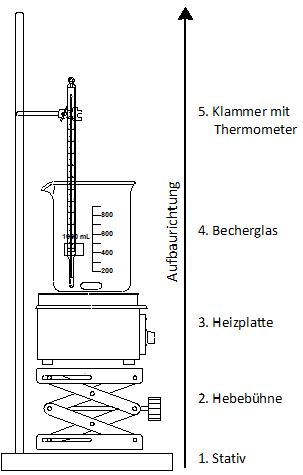
\includegraphics[width=0.8\textwidth]{img/Grundaufbau_Apparatur.png}
\end{minipage}
\begin{minipage}{0.55\textwidth}
		 Im Regelfall sollte eine Apparatur von "`unten nach oben"' aufgebaut werden. Die Arbeitsweise sichert den Halt und erleichter das strukturierte Auf- und Abbauen der Apparatur.
		 Ansonsten sollte man sich gerade in Angelegenheiten des Kühlens oder Heizens überlegen, wie die Höhe der Hebebühne einzustellen ist, um gegebenenfalls die Probe ohne Abbau der Messapparaturen zu erreichen.
\end{minipage}

\subsubsection{Schliffklemmen alias \textsc{Keck}-Clips}
Schliffklemmen bzw. \textsc{Keck}-Clips sichern die Verbindung zwischen Glasgeräten mit Normschliff. Diese Art von Schliffsicherung findet sich vorrangig im anorganischen und organischen Chemiepraktikum für den Aufbau größerer Apparaturen. Die Ausführung der Schliffklemmen ist verschiedenen Formen und Materialien zu finden. Eine häufig vertretende Form aus Kunststoff  sind die patentierten \textsc{Keck}-Clips.

\begin{figure}
	\begin{minipage}[b]{.45\textwidth} % [b] => Ausrichtung an \caption
		\centering
		\includegraphics[width=0.7\textwidth]{img/keck_clips}
		\caption{Skizze von \textsc{Keck}-Clips}
	\end{minipage}
	\hspace{.1\linewidth}% Abstand zwischen Bilder
	\begin{minipage}[b]{.45\textwidth} % [b] => Ausrichtung an \caption
		\centering
		\includegraphics[width=0.8\textwidth]{img/keck_clips_2}
		\caption{Beispielhafte Nutzung von \textsc{Keck}-Clips}
	\end{minipage}
\end{figure}
\FloatBarrier

\subsubsection{Muffen}
Stativmuffen sind einer der häufigsten verwendeten Bauteil im apparativen Labor. Sie werden vorzugsweise für die Befestigung von zylindrischen Stativteilen, wie einer Stativklemme oder einem Stativring.
\begin{figure}[h!]
	\centering
	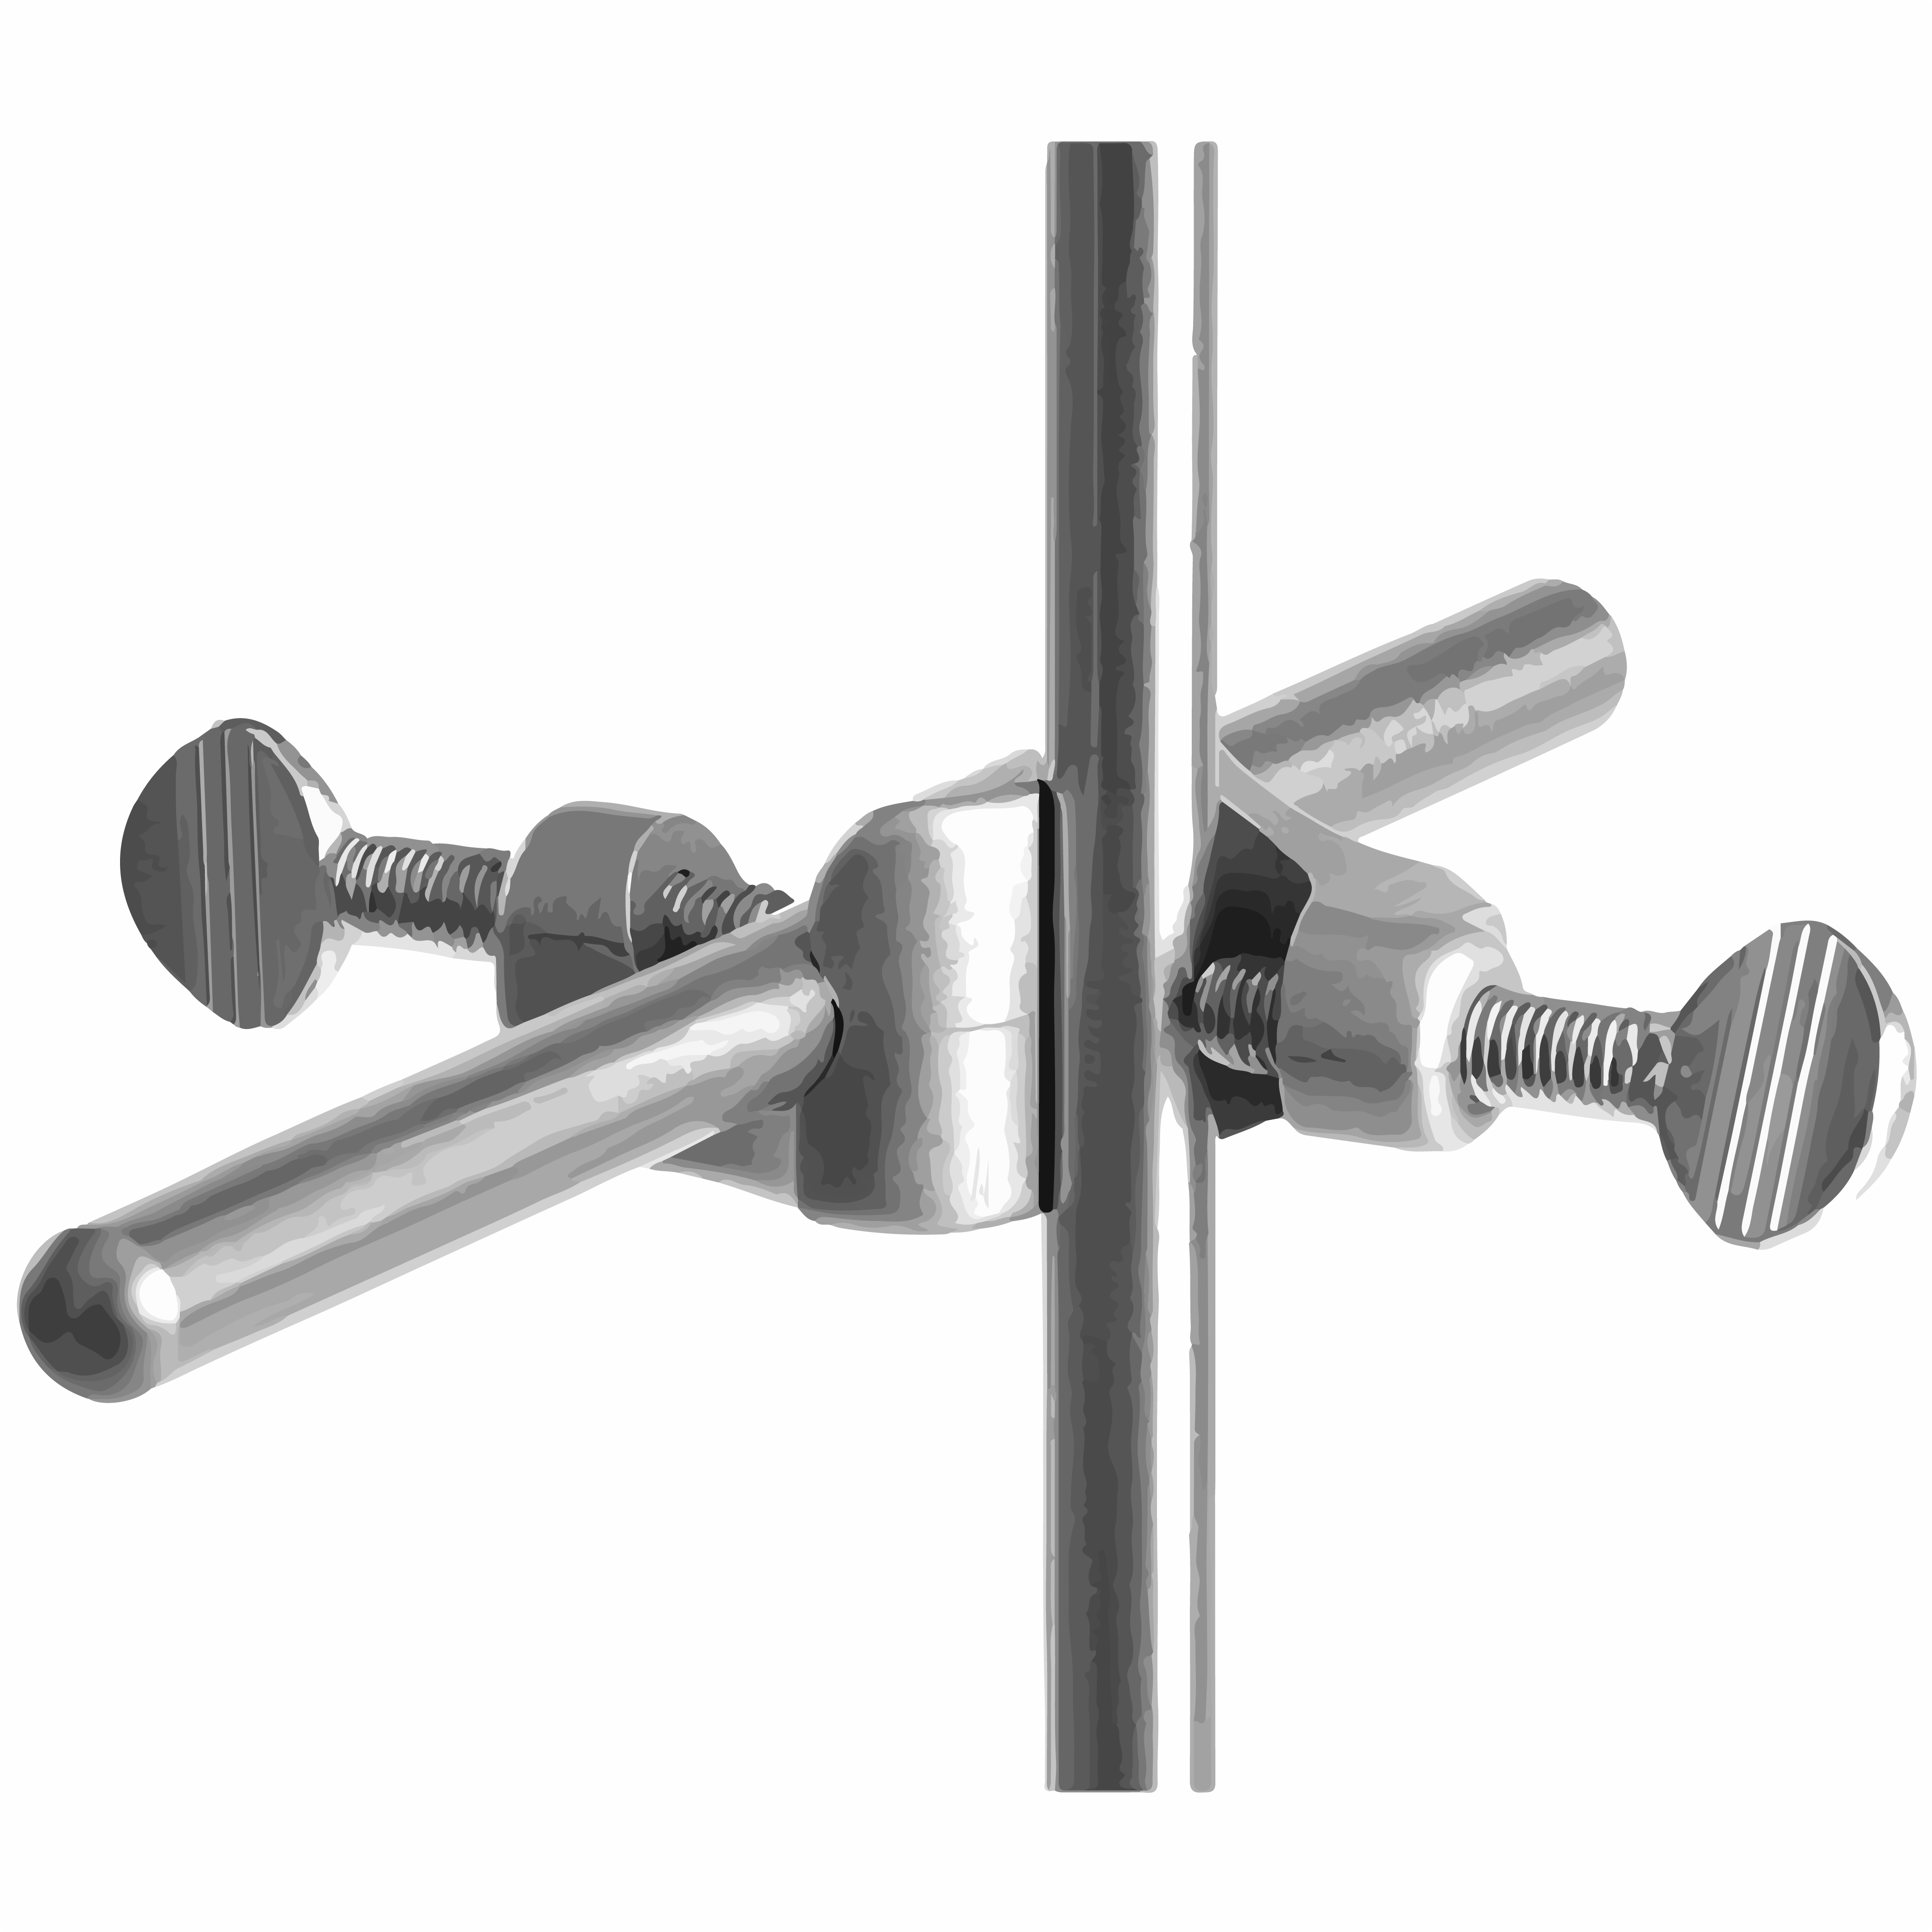
\includegraphics[width=0.5\textwidth]{img/muffe}
	\caption{Bild einer Stativmuffe}
	\label{fig:muffe}
\end{figure}
\FloatBarrier
%Ende

\subsubsection{Stative}
\subsubsection{Korkringe}

\subsection{Volumengefäß}
\subsubsection{Bechergläser}
\subsubsection{Rundkolben}
\subsubsection{Erlenmeyerkolben}
\subsubsection{Maßkolben}
\subsubsection{Bürette}

\subsection{Pipetten}
\subsubsection{Peleusball}
\subsubsection{Vollpipetten}
\subsubsection{Eppendorfpipetten}
\subsubsection{Hubkolbenpipette}

\subsection{Trichter}
\subsubsection{Flüssigkeitstrichter}
\subsubsection{Feststofftrichter}
\subsubsection{Tropftrichter}
\subsubsection{Scheidetrichter}

\subsection{Schläuche}
\subsubsection{Vakuumschläuche}
\subsubsection{Wasserschläuche}
\subsubsection{Oliven}

\subsection{Filter}
\subsubsection{Filterpapier}
\subsubsection{Fritte}
\subsubsection{Filternutsche}

\subsection{Waschflaschen}

\subsection{Rührer}
\subsubsection{Magnetrührwerk}
\subsubsection{Rührertypen}
\subsubsection{Rührermotor}

\subsection{Rückflusskühler}
\subsubsection{Dimrothkühler}
\subsubsection{Liebigkühler}

\subsection{Heizelemente}
\subsubsection{Wärmebad}
\subsubsection{Brenner}
\subsubsection{Heizpilz oder Heiznetz}
\subsubsection{Heizplatte}

\subsection{Pyknometer}

\subsubsection{Apparaturen zum Trocknen}
\subsubsection{Exsikkator}
\subsubsection{Trockenschrank}
\subsubsection{Muffelofen}

\subsection{Pumpen}
\subsubsection{Vakuumpumpe (Wasserstrahlpumpe)}
\subsubsection{Hubkolbenpumpe}
\subsubsection{Kreiselpumpe}

\subsection{Zusätzlich:}
\subsubsection{Beschriftung von Proben}
\subsection{Füllkörper}
\subsubsection{Schliffe und Schlifffett}
\subsubsection{Ultraschallbad}
\subsubsection{Eismaschine}